\documentclass{article}
\usepackage{algpseudocode,algorithm,algorithmicx}
\usepackage[usenames,dvipsnames,svgnames,table]{xcolor}
\usepackage{hyperref}
\usepackage{graphicx}

\begin{document}
    \title{\textcolor{blue}{\textbf{Problema 1 }}\\}
    \author{Daniel de la Cruz Prieto C211\\ David Orlando De Quesada Oliva C211\\Javier Dominguez C212} 
    \date{}
    \maketitle  

    \section{\underline{Orden del problema}} 

    Sean n casas en un vecindario y m tuber\'ias. Las tuber\'ias de agua subterr\'aneas conectan estas casas. Cada
    tuberı\'ia tiene cierta direcci\'on (el agua puede fluir solo en esta direcci\'on y no al rev\'es) y di\'ametro (que caracteriza
    la cantidad m\'axima de agua que puede manejar).
    \\[10pt]
    \noindent Para cada casa, hay como m\'aximo una tuber\'ia entrando y como m\'aximo una tuber\'ia saliendo de ella. Se quiere
    instalar tanques y grifos en las casas. Para cada casa con una tuber\'ia de agua saliente y sin una tuber\'ia de agua
    entrante, se debe instalar un tanque de agua en esa casa. Por cada casa con una tuber\'ia de agua entrante y
    sin una tuber\'ia de agua saliente, se debe instalar un grifo de agua en esa casa. Cada casa tanque transportar\'a
    agua a todas las casas que tengan una secuencia de tuber\'ias desde el tanque hasta ella. En consecuencia, cada
    casa de grifo recibir\'a agua procedente de alguna casa de tanque.
    \\[10pt]
    \noindent Para evitar que las tuber\'ias exploten una semana después tambi\'en se debe considerar el di\'ametro de las tuber\'ias.
    La cantidad de agua que transporta cada tanque no debe exceder el di\'ametro de las tuber\'ias que conectan un
    tanque a su correspondiente grifo. Se quiere encontrar la cantidad m\'axima de agua que se puede transportar de
    forma segura desde cada tanque hasta su grifo correspondiente. Dise\~ne un algoritmo que devuelva la cantidad
    m\'axima de agua que se puede trasnportar de forma segura desde cada tanque hasta su grifo correspondiente.
    La complejidad temporal de su algoritmo debe ser de \textit{O(n + m)}.
    
    \newpage
    \section{\underline{Soluci\'on}}

    Primero que todo consideremos el conjunto de casas del vecindario como los v\'ertices, y las tuber\'ias como las aristas de un grafo
    dirigido  $G$, las aristas tienen una funci\'on de capacidad (di\'ametro de la tuber\'ia) y los v\'ertices tienen a lo sumo $indegree = 1$
    y a lo sumo $outdegree$ = 1 por las restricciones del problema.\\\\

    Definici\'on: Una casa con tanque $u$ en el grafo $G$ es un $u \in V(G)$,\\ $indegree(u) = 0 \wedge outdegree(u) = 1$\\

    Definici\'on: Una casa con grifo $u$ en el grafo $G$ es un $u \in V(G)$,\\ $indegree(u) = 1 \wedge outdegree(v) = 0$\\

    Definici\'on: Diremos que a la casa con tanque $u$, en el grafo $G$, le corresponde la casa con grifo
     $v$, si existe un camino de $u$ a $v$ en $G$.\\

    Definici\'on: Diremos que a la casa con grifo $u$ en el 
    grafo $G$, le corresponde la casa con tanque $v$, si existe un camino de $u$ a $v$ en $G$.\\\\

    Proposici\'on 1: A cada casa con tanque $u \in V(G)$ le corresponde una \'unica casa con grifo $v \in V(G)$.\\

    Supongamos que a una casa con tanque $u \in V(G)$ le corresponde al menos dos casas con grifo, eso quiere decir
    que hay un camino de $u$ a cada una de dichas casas. Tomemos dos de dichas casas y los caminos $p_1, p_2$ de $u$
    a cada una de ellas, pueden ocurrir dos cosas con dichos caminos:\\\\

    $\bullet$ Los caminos $p_1$ y $p_2$ solo tienen en com\'un el v\'ertice $u$ (casa con tanque). En este caso
    el $outdegree(u) \geq 2$ (al menos tiene grado dos, pues solo tomamos estos dos caminos, pero pueden haber m\'as que
    solo tengan a $u$ como v\'ertice com\'un).\\

    $\bullet$ Los caminos $p_1$ y $p_2$ tienen en com\'un m\'as de un v\'ertice. En este caso comencemos recorriendo $p_1$ desde
    $u$, y sea $w$ el \'ultimo v\'ertice com\'un con $p_2$ en $p_1$, se cumple que $outdegree(w) \geq 2$ (pueden que hayan mas caminos
    que lleguen a $w$ por el mismo recorrido que $p_1, p_2$).\\\\

    En ambos casos llegamos a una contradicci\'on con las restricciones del problema, que es que $\forall x \in V(G), outdegree(x) \leq 1$. 
    Por tanto a cada casa con tanque $u$ le corresponde una \'unica casa con grifo $v$.\\\\

    Proposici\'on 2: A cada casa con grifo $u \in V(G)$ le corresponde una \'unica casa con tanque $v \in V(G)$.\\

    Supongamos que a la casa con grifo $u$ le corresponden al menos dos casas con tanque, eso quiere decir que hay al menos dos casas
    con tanque tal que hay un camino de cada una de ellas a la casa con grifo $u$. Tomemos dos de dichas casas y los caminos $p_1, p_2$,
     que van de cada una de ellas a la casa con grifo $u$, pueden ocurrir dos cosas con dichos caminos:\\\\

    $\bullet$ Los caminos $p_1$ y $p_2$ solo tienen en com\'un el v\'ertice $u$ (casa con grifo). En este caso
    el $indegree(u) \geq 2$ (al menos tiene grado dos, pues solo tomamos estos dos caminos, pero pueden haber m\'as que
    solo tengan a $u$ como v\'ertice com\'un)\\
 
    $\bullet$ Los caminos $p_1$ y $p_2$ tienen en com\'un m\'as de un v\'ertice. En este caso comencemos recorriendo $p_1$ y $p_2$ desde cada
    uno de sus v\'ertices iniciales hasta $u$, y tomemos el primer v\'ertice com\'un a ambos en dicho recorrido, ese v\'ertice que digamos es $w$
    cumple que $indegree(w) \geq 2$ (pueden que hayan mas caminos que lleguen a $w$)\\\\

    En ambos casos llegamos a una contradicci\'on con las restricciones del problema, que es que $\forall x \in V(G), indegree(x) \leq 1$. 
    Por tanto a cada casa con grifo $u$ le corresponde una \'unica casa con tanque $v$.\\\\

    Por las Proposiciones 1 y 2 se deduce que cada casa con grifo recibe agua de una sola casa con tanque, y una casa con tanque env\'ia agua a
    una sola casa con grifo. Que esto es que los pares $u,v \in V(G)$ tal que $u$ env\'ia agua a $v$, no tienen elementos repetidos\\\\\

    Proposici\'on 3: Entre cada casa tanque $u \in V(G)$ y su grifo correspondiente, $v \in V(G)$ hay un \'unico camino
    que va de $u$ a $v$ en $G$ y es un camino simple.\\

    Supongamos que hay al menos dos caminos que van de $u$ a $v$ en $G$. Tomemos dos de dichos caminos, $p_1$ y $p_2$, ambos caminos pueden cumplir solo las 
    siguientes condiciones:\\\\

    $\bullet$ Ambos empiezan en $u$ y el v\'ertice siguiente en ambos caminos es distinto, en este caso $outdegree(u) \geq 2$\\\\
    $\bullet$ Ambos tienen una serie de v\'ertices en com\'un y se separan en alg\'un punto del recorrido antes de llegar a $v$, 
    en este caso tomemos el \'ultimo v\'ertice com\'un a $p_1$ y $p_2$, denotemos ese v\'ertice como $w$, se cumple que $outdegree(w) \geq 2$\\\\

    En ambos casos llegamos a una contradicci\'on con las restricciones del problema, que es que $\forall x \in V(G), outdegree(x) \leq 1$. 
    Por tanto para toda casa con tanque $u$ que env\'ia agua a su correspondiente casa con grifo $v$, se cumple que existe un \'unico camino de $u$ a $v$.\\\\

    Ahora supongamos que ese camino que denotaremos como $p_i$ no es simple, eso quiere decir que hay un ciclo en dicho camino, empezemos a recorrer $p_i$ hasta 
    que lleguemos al primer v\'ertice $x$ que est\'a en dicho ciclo, la arista que usamos para llegar a \'el no estaba en el ciclo y aporta 1 de $indegree$ a $x$,
     y la otra arista $y$, que cierra el ciclo en $x$ aporta 1 de $indegree$, por lo que $indegree(x) = 2$, lo que es una contradicci\'on con las restricciones del problema.\\\\

    Por tanto, el \'unico camino entre $u$ y $v$ en $G$, es simple.\\\\

    Debido a que las proposiciones previamente analizadas son ciertas, el vecindario(casas y tuber\'ias) representado utilizando un grafo dirigido $G$, quedar\'ia de la siguiente forma:\\\\

    \begin{figure}[h]
        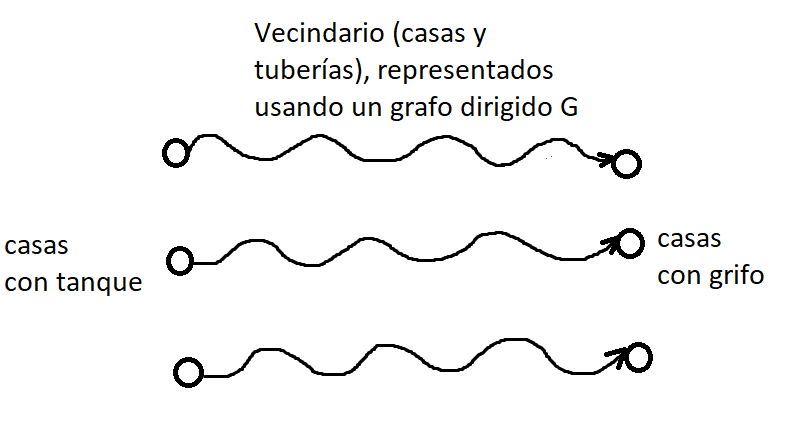
\includegraphics[scale = 0.5]{Image1Problem1.png}
        \centering
    \end{figure}

    O sea, el vecindario represenado utilizando un grafo dirigido $G$, queda formando varias componentes conexas en el grafo $G$,
    donde cada un de dichas componentes conexas representa un \'unico camino simple que va de una casa con tanque, a su correspondiente
    casa con grifo.\\\\

    \section{\underline{Complejidad Temporal}}
    La complejidad de nuestro algoritmo se basa en la complejidad del DFS $O(n+m)$.Lo \'unico que le agregamos al DFS
    es ir actualizando  el m\'inimo de las capacidad de las aristas que participan en un camino desde un tanque hasta un 
    grifo lo cual no afecta la complejidad temporal del mismo. Luego hacemos un recorrido por cada v\'ertice v del array max
    para imprimir las casa que son tanque con la m\'axima capacidad correspondiente que se puede transportar de forma segura 
    desde el mismo hasta un grifo,lo cual tiene complejidad $O(n)$.Por lo cual mi algoritmo tiene complejidad $O(n+m)$.
    
    \newpage
    \section{\underline{Pseudoc\'odigo}}
    \begin{algorithm}
        \caption{Calcular la capacidad máxima de agua que se puede transportar de forma segura desde cada tanque hasta su grifo correspondiente}
        \textbf{Solve($G$)\\}
        1-\hspace*{1em}max=[] -array donde voy tener para cada v\'ertice en caso que sea tenga la capacida m\'axima a transportar\\
        2-\hspace*{1em}DFS-Visit($G,u,min,ficvertex)$\\ 
        3-\hspace*{2em}u $\leftarrow$ visited \\
        4-\hspace*{2em}$time=time+1$ \\  
        5-\hspace*{2em}for each v $\in$ $Adj[u]$\\
        6-\hspace*{3em}do if v not visited\\
        7-\hspace*{4em}$\pi[v] \leftarrow u$\\
        8-\hspace*{4em}do if $c(u,v)< min$\\
        9-\hspace*{4em}$min=c(u,v)$\\
        10-\hspace*{4em}DFS-Visit(G,v,min)\\
        11-\hspace*{2em}do $if pi[u]=ficvertex$\\
        12-\hspace*{3em}max[u]=min\\        
        13-\hspace*{2em}return\\\\
        14-\hspace*{1em}for i in max\\
        15-\hspace*{2em}if $max[i] != \infty $\\
        16-\hspace*{3em}print(i,pi[i])\\
        
        %Me parece que seria mejor si lo agrego a una lista y despues pregunto por lista.count para no modificar mucho del codigo
        
    \end{algorithm}
\end{document}